\chapter{弗里德曼動力學與狀態方程}

\lectureoverview{必須區分均勻膨脹與局部束縛系統的物理，也必須區分內在幾何與嵌入空間中的形狀。確立這些區分後，宇宙學原理便將時空度規簡化為一個尺度因子 \(a(t)\) 和一個曲率標記 \(k\)。愛因斯坦方程的時間－時間分量隨即成為弗里德曼能量方程。要解出它，還需要壓力與能量密度之間的物質關係。絕熱熱力學與狀態方程 \(P=w\rho\) 給出 \(\rho\propto a^{-3(1+w)}\)，將物質、輻射與真空能統一在同一個架構中。}

\section{釐清物理圖像的問題}

\subsection{空間會在視界之前重複嗎？}

有限的平直宇宙可以表示為一個週期性單元。如果這個單元小於可觀測區域，光便能穿越它，天空中也會出現同一批結構的重複影像。要偵測這些重複，遠比認出一個熟悉的星系困難：影像來自不同方向與不同時期，也會受到宇宙演化的影響。儘管如此，週期性拓撲仍會帶來可觀測的效應。

\begin{classroomqa}
\audiencequestion{整個宇宙有可能比可觀測宇宙還小嗎？}
\lecturerresponse{自然的候選方案是將空間週期性地識別成環面。如此一來，我們看到的便是同一物理區域的重複副本；打個比方，就像從後門看見自己。搜尋相應的宇宙週期性，至今沒有找到支持證據，但確實對較小的基本單元施加了限制。這種可能性在幾何上自洽，但現有證據並不支持宇宙小於我們已觀測到的區域。 \lecturetimestamp{00:01:17--00:02:33}}
\end{classroomqa}

\subsection{膨脹不會拉開束縛系統}

宇宙膨脹描述的是自由運動物質在平均宇宙幾何中的大尺度運動。它不是一條要求所有固有長度都必須增加的普遍指令。電磁力束縛原子，引力束縛行星系統，而普通分子力束縛固體物件。在這些尺度上，這些交互作用遠比宇宙學修正強得多。

\begin{classroomqa}
\audiencequestion{膨脹是由暗能量造成的嗎？為什麼原子或行星軌道不會隨空間一起膨脹？}
\lecturerresponse{暗能量被發現之前，人們就已知道宇宙正在膨脹。暗能量會使膨脹加速，因而改變膨脹；它並非膨脹的定義，也不是膨脹最初的成因。束縛系統不會跟著哈伯流膨脹，因為局部作用力占主導地位。加速膨脹的背景可能對原子或軌道造成極微小的擾動，但一般的束縛作用會使系統回到幾乎不變的平衡狀態，而不會讓它散開。 \lecturetimestamp{00:02:36--00:06:50}}
\end{classroomqa}

\subsection{時變幾何中的能量}

剩下的疑問不在於力，而在於能量帳目。如果束縛軌道持續抵抗微小的宇宙學擾動，所需的能量從何而來？這個問題把靜態背景中的守恆定律，套用到不具有全域時間平移對稱性的時空上。

\begin{classroomqa}
\audiencequestion{局部束縛作用抵抗膨脹時，能量從何而來？}
\lecturerresponse{靜態世界中的能量守恆源自時間平移不變性：實驗在時間上平移後，背景及其定律看起來仍然相同。膨脹時空在這種全域意義上不具有時間平移不變性，因此整個宇宙未必有一個守恆的總能量。局部應力－能量守恆仍然成立，稍後會以連續方程的形式出現。失效的是一種天真的主張：幾何改變時，必定有一個全域定義的宇宙能量維持不變。 \lecturetimestamp{00:06:52--00:09:24}}
\end{classroomqa}

\subsection{均勻性是粗粒化後的描述}

宇宙學原理適用於特定尺度。封閉房間中的空氣在房間尺度上可能近乎均勻，但在分子尺度上則呈現顆粒性。宇宙也包含行星、星系、星系團與密度漲落。均勻性與各向同性指的是宇宙在足夠大距離上的平均行為；在這些尺度上，那些結構已不再選定某個位置或方向。

\begin{classroomqa}
\audiencequestion{小尺度的束縛結構會與均勻性和各向同性矛盾嗎？}
\lecturerresponse{不會。小尺度上並非嚴格均勻，就像看清單個分子時，空氣也不再均勻一樣。在數億光年及更大的尺度上，觀測到的分布近似均勻，且不依賴方向。在我們可觀測區域之外，均勻性仍是一項假設；其推論必須接受檢驗，而不是已確立的事實。 \lecturetimestamp{00:09:27--00:10:55}}
\end{classroomqa}

\section{作為度規陳述的均勻性與各向同性}

均勻性與各向同性首先是幾何陳述，其次才是動力學陳述。愛因斯坦方程會告訴我們幾何如何隨時間變化。首先，我們必須說明在任一時刻允許哪些空間幾何。

\begin{classroomqa}
\audiencequestion{均勻性與各向同性在數學上代表什麼？}
\lecturerresponse{用度規描述空間，並選取以某一點為中心的座標 \(x^i\)。再選取以另一點為中心的座標 \(y^i\)。均勻性表示存在一種變換，可以移動原點，同時保持度規的函數形式不變。於是，每一點在幾何上都與其他各點等價。各向同性則進一步要求空間繞每一點都具有旋轉對稱性，因此沒有任何方向特別受到偏好。 \lecturetimestamp{00:11:13--00:14:26}}
\end{classroomqa}

\begin{definition}
若存在等距變換，能將任一點映到其他任一點，則空間是\emph{均勻的}。若繞某一點旋轉後，幾何保持不變，則空間在該點\emph{各向同性}。均勻且各向同性的空間，既沒有偏好的位置，也沒有偏好的方向。
\end{definition}

歐幾里得平面清楚呈現了這個定義。在笛卡兒座標中，
\begin{equation}
ds^2=dx_1^2+dx_2^2.
\label{eq:c04-flat-metric}
\end{equation}
將原點平移常數 \(a_1\) 和 \(a_2\)：
\begin{equation}
y_1=x_1+a_1,
\qquad
y_2=x_2+a_2.
\label{eq:c04-flat-translation}
\end{equation}
由於 \(dy_i=dx_i\)，平移後的度規為
\begin{equation}
ds^2=dy_1^2+dy_2^2.
\end{equation}
標記各點的符號變了，但距離規則沒有改變。這是均勻性最簡單的例子。旋轉也會保持度規不變，因此平面同樣具有各向同性。

球面的情況較不直觀，只是因為座標沒那麼方便。以南極為原點，單位二維球面可寫成
\begin{equation}
d\Omega_2^2=dr^2+\sin^2 r\,d\theta^2.
\label{eq:c04-sphere-metric}
\end{equation}
將球面旋轉，讓東極成為新的原點。座標變換雖然繁複，結果仍是方程式~\eqref{eq:c04-sphere-metric}。圓球面上沒有任何一點在幾何上特別突出。

\begin{classroomqa}
\audiencequestion{週期識別的平坦環面是否同時具有均勻性和各向同性？}
\lecturerresponse{它在平移下具有均勻性：週期單元中的每一點都具有相同的局部幾何。但它並非完全各向同性，因為識別方式選定了偏好的週期方向與長度。沿其中一條軸觀察，與沿一般斜向觀察，在全域上並不相同。因此，環面清楚展現了有均勻性但不完全各向同性的情況。 \lecturetimestamp{00:20:18--00:21:30}}
\end{classroomqa}

觀測到的大尺度均勻性，支持我們在視界內採用宇宙學原理。將它延伸至可觀測區域之外，是一項假設，而非直接觀測所得。我們接受這項假設，是因為它給出定義明確的幾何，其推論可以拿來與資料比對。

\section{內在幾何與嵌入}

提到球面空間時，人們很容易想像一個放在大房間裡的氣球表面。這種圖像或許有助於作圖，但周圍的房間並不屬於宇宙學所要表達的內容。真正重要的是\emph{內在}幾何：它由始終留在空間內的觀察者所能測量的距離與角度構成。

\subsection{封閉的一維世界}

考慮一個封閉的一維世界。我們可以把它畫成圓形、圓角正方形，或花生形的環。被限制在線上的居民只能測量沿線距離。如果兩個環的總周長相同，即使圖形看起來完全不同，居民所測得的內在幾何仍然相同。

\begin{figure}[htbp]
\centering
\includegraphics[width=0.72\textwidth]{lecture_04_figure_05.png}
\caption{圓形與變形的封閉環，用來區分內在幾何與嵌入形狀。這張較晚拍攝的畫面保留了先前討論時所畫的圖；相關內容出現在 00:23:21--00:25:59。}
\label{fig:c04-intrinsic-board}
\lectureframe{00:59:54.899}
\end{figure}

所有一維度規在局部上都是平坦的。一小段繩子可以在不拉伸的情況下拉直，因此它在周圍平面中呈現的彎曲屬於外在彎曲，而非內在曲率。封閉環有一個全域模數，也就是它的周長；但它沒有任何內在的局部彎曲，可供生活在其中的一維居民測量。

\begin{figure}[htbp]
\centering
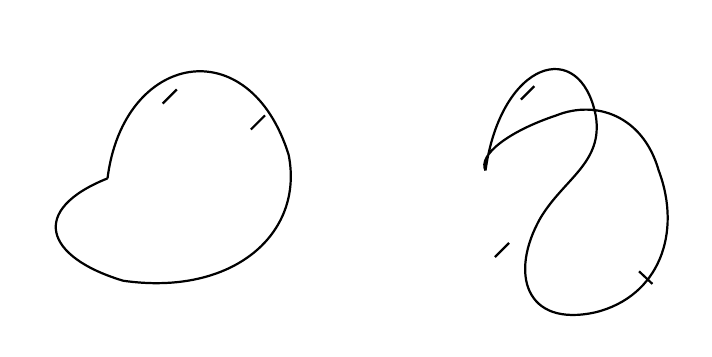
\begin{tikzpicture}[scale=1.0]
\draw[line width=0.8pt] (0,0)
  .. controls (0.2,1.6) and (1.8,1.9) .. (2.3,0.3)
  .. controls (2.5,-0.7) and (1.6,-1.5) .. (0.2,-1.3)
  .. controls (-0.8,-1.0) and (-1.0,-0.4) .. (0,0);
\draw[line width=0.8pt] (0.70,0.95) -- (0.88,1.13);
\draw[line width=0.8pt] (1.82,0.62) -- (2.00,0.80);

\draw[line width=0.8pt] (4.8,0.1)
  .. controls (5.0,1.5) and (6.0,1.8) .. (6.2,0.8)
  .. controls (6.3,0.2) and (5.8,0.0) .. (5.5,-0.5)
  .. controls (5.1,-1.2) and (5.3,-1.9) .. (6.2,-1.7)
  .. controls (7.0,-1.5) and (7.3,-0.7) .. (7.0,0.1)
  .. controls (6.8,0.8) and (6.2,1.0) .. (5.7,0.8)
  .. controls (5.1,0.6) and (4.7,0.3) .. (4.8,0.1);
\draw[line width=0.8pt] (5.25,1.00) -- (5.42,1.17);
\draw[line width=0.8pt] (5.10,-0.82) -- (4.92,-1.00);
\draw[line width=0.8pt] (6.75,-1.18) -- (6.92,-1.34);
\end{tikzpicture}
\caption{圓形與變形環的清晰重繪。周長相同，表示一維內在幾何相同。}
\label{fig:c04-intrinsic-redraw}
\end{figure}

\begin{classroomqa}
\audiencequestion{有限線段也算是同一類的一維空間嗎？}
\lecturerresponse{不算。線段有兩個端點，封閉環則沒有端點。這種拓撲差異是內在的，無法透過將任一物件彎入更大的空間而消除。拓撲一旦固定，線段由其長度決定，封閉環則由其周長決定。 \lecturetimestamp{00:26:00--00:26:39}}
\end{classroomqa}

\subsection{嵌入為何有用但非必要}

我們將一維圓嵌入二維空間，並將二維球面嵌入三維空間，以便將它們視覺化。這種模式容易讓人以為，討論三維球面之前必須先有第四個歐幾里得維度。這種要求反映的是人類的視覺想像能力，而非數學上的必要性。我們的視覺系統演化出來，是為了在三維空間中行動；透過座標與度規，我們可以超越這個限制進行推理，而不必構造一個字面意義上的外部視角。

\begin{classroomqa}
\audiencequestion{額外的空間維度可能存在，只是小到無法觀測嗎？}
\lecturerresponse{可能。幾何並不要求所有維度都具有相同的可觀測尺度。緊緻維度的尺度可能遠小於日常經驗所能探測的範圍。不過，眼前的要點更簡單：無論額外維度是否在物理上存在，定義我們三維空間的內在度規，都不需要嵌入維度。 \lecturetimestamp{00:29:55--00:30:12}}
\end{classroomqa}

\begin{classroomqa}
\audiencequestion{被限制在彎曲線上的居民，如何知道那條線是否彎曲？}
\lecturerresponse{只靠內在測量，牠無從得知。想像光與物質都被限制在光纖中。在不拉伸光纖的情況下將它彎曲，會改變嵌入方式，卻不會改變沿光纖測得的距離或訊號傳播時間。只有逃逸到周圍空間的訊號，才能揭示外在的彎曲。 \lecturetimestamp{00:30:15--00:31:14}}
\end{classroomqa}

這個思想實驗可以具體實行。受限於光纖中的生物可以發射訊號，例如能量足夠高的光子。只有當訊號逃出光纖，之後又沿著一維度規中不存在的路徑返回時，牠才能發現外部方向。同樣地，普通空間具有三個大尺度維度，歸根究柢是實驗結果，而非從人類的想像能力推導而來。

\begin{classroomqa}
\audiencequestion{如果每一種一維空間在局部上都是平坦的，那麼每一種二維空間也都必須在局部上平坦嗎？}
\lecturerresponse{不必。一張捲成圓柱面的薄片仍具有內在平坦性：它可以在不拉伸的情況下展開。半球面則無法在不拉伸或撕裂的情況下展平到平面上，因此具有內在曲率。每一個足夠小的區域看起來都近似歐幾里得，但在有限尺度上會出現可測量的偏差。圓柱面與球面的差異，正是外在彎曲與內在曲率的差異。 \lecturetimestamp{00:31:14--00:35:00}}
\end{classroomqa}

\begin{classroomqa}
\audiencequestion{內在曲率是否必然表示存在引力場？}
\lecturerresponse{在廣義相對論中，時空曲率是不依座標選擇的潮汐引力表現。因此，宇宙學空間曲率 \(k/a^2\) 屬於引力幾何的一部分，而不只是想像中外部空間的彎曲。物質透過愛因斯坦方程影響曲率，但不應將這個說法進一步簡化成「只有物質所在之處才有曲率」：真空時空也能具有韋爾曲率，例如恆星外部或引力波中的曲率。 \lecturetimestamp{00:35:01--00:35:51}}
\end{classroomqa}

現在採用大尺度理想化。對恆星、星系、星系團與局部不規則結構取平均，就像描述地球為圓形時會忽略山脈一樣。所得的空間幾何假設為均勻且各向同性。在這些假設下，常曲率的可能性有三種：平坦、球面與雙曲。

\section{FRW 度規假設與三種曲率情形}

對稱性假設將幾何簡化為一個隨時間變化的尺度因子，以及一個離散的曲率符號。在共動座標中，弗里德曼－勒梅特－羅伯遜－沃克（FRW）度規假設為
\begin{equation}
ds^2=-dt^2+a(t)^2\,d\Sigma_k^2,
\qquad
k\in\{-1,0,+1\}.
\label{eq:c04-frw}
\end{equation}
時間座標是共動觀察者的固有時。均勻性允許 \(a\) 隨時間變化，但不隨位置變化；各向同性則不允許存在偏好的空間方向。

\begin{figure}[htbp]
\centering
\includegraphics[width=0.74\textwidth]{lecture_04_figure_02.png}
\caption{三種常曲率空間度規列在共同的尺度因子之下。這張畫面拍攝得較晚，當時黑板上已經寫有其他內容，但仍保留了 00:40:23--00:42:42 的度規討論。}
\label{fig:c04-frw-board}
\lectureframe{00:45:48.386}
\end{figure}

使用徑向座標 \(r\) 與單位二維球面度規 \(d\Omega_2^2\)，三種歸一化空間度規為
\begin{align}
d\Sigma_0^2 &= dr^2+r^2d\Omega_2^2,
&& k=0,
\label{eq:c04-flat-space}\\
d\Sigma_{+1}^2 &= dr^2+\sin^2 r\,d\Omega_2^2,
&& k=+1,
\label{eq:c04-spherical-space}\\
d\Sigma_{-1}^2 &= dr^2+\sinh^2 r\,d\Omega_2^2,
&& k=-1.
\label{eq:c04-hyperbolic-space}
\end{align}
因此在固定時刻，空間可以是平坦、具有正曲率或具有負曲率。乘上 \(a(t)^2\) 會以相同因子改變所有空間距離，同時保留歸一化後的形狀。

考慮兩個共動距離固定為 \(\Delta\chi\) 的星系。它們的物理距離為
\begin{equation}
D(t)=a(t)\Delta\chi.
\end{equation}
對兩邊微分並消去 \(\Delta\chi\)，得到
\begin{equation}
\dot D=\dot a\,\Delta\chi
      =\frac{\dot a}{a}D
      =H(t)D,
\qquad
H(t)\equiv\frac{\dot a}{a}.
\label{eq:c04-hubble-law}
\end{equation}
因此，哈伯定律在運動學上源自均勻的尺度變化。哈伯參數可以隨時間改變，但在任一固定的宇宙時刻，它在各處都相同。

\section{從愛因斯坦方程推導弗里德曼方程}

度規告訴我們如何測量距離，卻沒有說明 \(a(t)\) 如何演化。彎曲時空需要愛因斯坦方程。若逐一計算所有克里斯托費爾符號與曲率分量，反而會模糊物理論證，因此我們採用對稱性所決定的形式，並聚焦於時間－時間分量。

在 \(c=1\) 的單位制下，並暫時略去宇宙學常數，完整的張量方程為
\begin{equation}
G_{\mu\nu}
\equiv
R_{\mu\nu}-\frac12 g_{\mu\nu}R
=8\pi G\,T_{\mu\nu}.
\label{eq:c04-einstein}
\end{equation}
幾何量位於等式左側；能量密度、動量密度、壓力與應力則位於右側。因子 \(1/3\) 不屬於完整的張量方程。只有將時間－時間分量化為弗里德曼形式後，這個因子才會出現。

\begin{figure}[htbp]
\centering
\includegraphics[width=0.78\textwidth]{lecture_04_figure_03.png}
\caption{愛因斯坦方程黑板內容的中間狀態。幾何項的左側清晰可見，物質張量尚無法辨識，顯示的歸一化也不完整。推導所用的標準完整張量方程記於方程式~\eqref{eq:c04-einstein}。}
\label{fig:c04-einstein-board}
\lectureframe{00:48:19.394}
\end{figure}

對於在共動座標中靜止的均勻流體，
\begin{equation}
T_{00}=\rho.
\label{eq:c04-energy-density}
\end{equation}
時間－時間分量的愛因斯坦張量有一項值得注意的結構性質：其中的二階導數會相消，留下與一階時間導數平方成正比的一項，以及一項來自空間曲率：
\begin{equation}
G_{00}=3\left[
\left(\frac{\dot a}{a}\right)^2+\frac{k}{a^2}
\right].
\label{eq:c04-g00}
\end{equation}
將方程式~\eqref{eq:c04-energy-density}和\eqref{eq:c04-g00}代入方程式~\eqref{eq:c04-einstein}，即可得到第一個弗里德曼方程，
\begin{equation}
\boxed{
\left(\frac{\dot a}{a}\right)^2+\frac{k}{a^2}
=\frac{8\pi G}{3}\rho
}.
\label{eq:c04-friedmann}
\end{equation}
也可以寫成
\begin{equation}
H^2=\frac{8\pi G}{3}\rho-\frac{k}{a^2}.
\label{eq:c04-friedmann-energy}
\end{equation}
方程式~\eqref{eq:c04-friedmann-energy}的形式，恰好與先前牛頓力學論證所得的形式相同。在那個論證中，積分常數被解釋為一團物質的總機械能，或其逃逸條件。廣義相對論則將內在空間曲率置於相同的數學位置。這種一致性並非偶然：在足夠小的區域內，曲率效應可以忽略，相對論宇宙學必須重現局部的牛頓力學行為。相對論也釐清了 \(\rho\) 代表總能量密度，因此相對論性粒子與光子也會產生引力，這些效應在非相對論性的質量密度論證中會被忽略。

\begin{classroomqa}
\audiencequestion{為什麼度規中沒有混合空間與時間的項？}
\lecturerresponse{混合項會表現得像是相對於共動觀察者存在一個偏好的空間向量或流動方向。嚴格的均勻性與各向同性不允許有這樣的方向。因此，在與宇宙物質相適應的座標中，位移向量為零，度規便呈現方程式~\eqref{eq:c04-frw}所示的區塊對角形式。只要所假設的對稱性維持不變，這就不是額外的動力學假設，而是幾何上的必然結果。 \lecturetimestamp{00:58:27--00:59:08}}
\end{classroomqa}

\begin{classroomqa}
\audiencequestion{為什麼只看時間－時間分量就足夠？二階導數到哪裡去了？}
\lecturerresponse{均勻且各向同性的度規假設中，只有一個未知函數 \(a(t)\)。混合分量化為恆等式，而空間分量則與時間－時間方程及應力－能量守恆相關。可以將它們合併成一個含有 \(\ddot a\) 的加速度方程，但時間－時間分量的愛因斯坦張量很特殊：二階導數項會相消，留下方程式~\eqref{eq:c04-friedmann}所示的一階能量方程。這一條非平凡方程，加上物質的演化定律，便足以決定唯一的幾何自由度。 \lecturetimestamp{00:59:09--01:00:56}}
\end{classroomqa}

\section{宇宙的組成如何稀釋}

除非知道 \(\rho\) 如何隨 \(a\) 變化，弗里德曼方程就不是封閉的。幾何已提供一條方程；宇宙中的物質還必須提供第二個關係。

對非相對論性物質而言，共動體積內的粒子數固定，而物理體積則按 \(a^3\) 增大。忽略粒子微小的動能，
\begin{equation}
\rho_{\mathrm m}(a)=\frac{\rho_{\mathrm m,0}}{a^3}.
\label{eq:c04-matter-scaling}
\end{equation}
可以在任何方便的參考時期將歸一化 \(a=1\) 設定為所需數值；能直接比較的只有尺度因子比值。

\begin{classroomqa}
\audiencequestion{如果平坦宇宙是無限的，那麼當 \(a\) 在大爆炸之際趨近於零，代表什麼？}
\lecturerresponse{只要 \(a\) 非零，無限平坦空間就始終是無限的；所有有限的共動距離都會乘上同一個縮小因子。在平坦情況下，\(a\) 的絕對歸一化可以任意選定，因此只有 \(a(t_2)/a(t_1)\) 具有不變的意義。對於封閉的球形宇宙，\(a\) 自然代表其曲率半徑；對於雙曲宇宙，則設定曲率半徑。極限 \(a\to0\) 表示宇宙學奇點，而不是外部空間中一個普通的有限球體。 \lecturetimestamp{01:05:06--01:05:53}}
\end{classroomqa}

輻射會以兩種方式損失能量。它的數密度隨體積的倒數下降，而且每個光子的波長會隨 \(a\) 成比例拉長，使光子能量再減少一個 \(a^{-1}\) 的因子。因此
\begin{equation}
\rho_{\mathrm r}(a)=\frac{\rho_{\mathrm r,0}}{a^4}.
\label{eq:c04-radiation-scaling}
\end{equation}
在往過去回推時，\(a^{-4}\) 的增長速度比 \(a^{-3}\) 更快，所以即使物質在較晚時期占主導，輻射在足夠早的時期仍會占主導。

若宇宙只有物質與輻射兩種成分，\(k\) 的正負便與宇宙未來密切相關：\(k=+1\) 允許宇宙再坍縮；\(k=0\) 是臨界情況，宇宙永遠膨脹但逐漸減速；\(k=-1\) 則使宇宙永遠膨脹，而曲率最終變得重要。暗能量打破了這種簡單關聯。封閉宇宙可以永遠膨脹，而空間平坦與否本身並不能決定宇宙的最終命運。

\section{狀態方程與連續性定律}

與其為每一種物質都背下一條稀釋規則，不如用狀態方程描述物質。這套做法分為兩步：先根據給定的壓力與能量密度關係，推導 \(\rho(a)\)；再從物質、輻射或真空的微觀物理，決定這個關係。本講只需要第一步。

壓力是動量通量。分子撞上盒壁後反轉動量，進而推動盒壁；粒子速度越快，傳遞的動量越多，產生的壓力也越大。因此，一旦指定物質種類，能量密度與壓力就不能各自獨立選定。對於簡單的宇宙學成分，我們寫成
\begin{equation}
P=w\rho,
\label{eq:c04-equation-state}
\end{equation}
其中 \(w\) 是無因次量，採用 \(c=1\) 的單位制。冷物質的壓力可忽略，因此 \(w=0\)。輻射則有 \(w=1/3\)；其中的因子 \(1/3\) 反映了對三個空間方向取平均。

\begin{figure}[htbp]
\centering
\includegraphics[width=0.82\textwidth]{lecture_04_figure_06.png}
\caption{黑板整理了物質與輻射的標度關係，並將狀態方程寫成 \(P=W\rho\)。我們採用慣例，以小寫字母 \(w\) 表示。}
\label{fig:c04-equation-state-board}
\lectureframe{01:15:08.166}
\end{figure}

\subsection{共動盒中的熱力學}

取一個共動盒，其物理體積為 \(V\)、能量密度為 \(\rho\)，總能量為
\begin{equation}
E=\rho V.
\end{equation}
熱力學第一定律為
\begin{equation}
dE=T\,dS-P\,dV.
\end{equation}
宇宙膨脹視為絕熱過程，因此對這個共動盒有 \(dS=0\)，並且
\begin{equation}
dE=-P\,dV.
\label{eq:c04-adiabatic-first-law}
\end{equation}
負號表示膨脹中的系統會對外做功，並失去內能。另對 \(E=\rho V\) 微分，可得
\begin{equation}
dE=\rho\,dV+V\,d\rho.
\end{equation}
令兩個表示式相等，
\begin{align}
\rho\,dV+V\,d\rho&=-P\,dV,\\
V\,d\rho&=-(\rho+P)\,dV.
\label{eq:c04-volume-continuity}
\end{align}
代入 \(P=w\rho\)，可得
\begin{equation}
\frac{d\rho}{\rho}=-(1+w)\frac{dV}{V}.
\end{equation}
積分後得到
\begin{equation}
\rho\propto V^{-(1+w)}.
\end{equation}
由於共動體積按 \(V\propto a^3\) 成比例變化，
\begin{equation}
\boxed{\rho(a)\propto a^{-3(1+w)}}.
\label{eq:c04-density-scaling}
\end{equation}
以微分形式表示，同一關係就是局部能量守恆方程
\begin{equation}
\dot\rho+3H(\rho+P)=0.
\label{eq:c04-continuity}
\end{equation}
即使變動的宇宙幾何未必允許全宇宙存在守恆的總能量，這條局部守恆定律仍然精確成立。

立即可得兩個熟悉的情況：
\begin{align}
w=0
&\quad\Longrightarrow\quad
\rho_{\mathrm m}\propto a^{-3},\\
w=\frac13
&\quad\Longrightarrow\quad
\rho_{\mathrm r}\propto a^{-4}.
\end{align}
輻射多出的反比次方，正是宇宙紅移在熱力學上的表現。

\begin{classroomqa}
\audiencequestion{今天宇宙中還有哪些輻射？}
\lecturerresponse{課堂討論主要指的是宇宙微波背景，也就是熾熱早期宇宙遺留下來的光子背景。如今輻射只占宇宙總能量密度的一小部分，但其 \(a^{-4}\) 標度關係表示，只要將方程式往過去回推得夠遠，輻射便會超過物質。現今各成分的精確比例來自觀測，這項標度論證並不需要這些數值。 \lecturetimestamp{01:26:53--01:28:34}}
\end{classroomqa}

\section{真空能與「曲率決定命運」規則的失效}

暗能量的狀態方程為
\begin{equation}
P=-\rho,
\qquad
w=-1.
\label{eq:c04-vacuum-eos}
\end{equation}
負壓就是張力：盒中的內容物不是向外推盒壁，而是向內拉盒壁。拉伸的彈簧是常見的張力物體，但這只是一種類比，並非真空能的微觀模型。

\begin{classroomqa}
\audiencequestion{負壓與絕對零度有關嗎？}
\lecturerresponse{兩者一般而言並沒有簡單的關聯。將普通物質冷卻至零溫，本身不會產生宇宙學狀態方程 \(P=-\rho\)。這段討論有助於區分熱壓力與真空應力：真空能的特徵是洛倫茲不變的應力－能量，其空間分量表現為負壓。真空能的微觀起源則是另一個問題。 \lecturetimestamp{01:31:01--01:31:46}}
\end{classroomqa}

將\(w=-1\)代入方程~\eqref{eq:c04-density-scaling}，可得
\begin{equation}
\rho_\Lambda\propto a^0=\text{constant}.
\label{eq:c04-vacuum-density}
\end{equation}
共動區域膨脹時，其體積與真空總能量同步增加，因此單位體積的能量維持不變。方程~\eqref{eq:c04-adiabatic-first-law}中的功項正是這種行為的原因，因為\(P\)為負。一旦存在這類成分，正空間曲率便不再足以保證宇宙重新坍縮。

\begin{classroomqa}
\audiencequestion{暗物質、黑洞和其他緻密天體如何納入？}
\lecturerresponse{在遠大於彼此間距的尺度上，任何隨機速度都很小的非相對論性成分，都會計入無壓物質密度。這包括普通物質、冷暗物質，以及黑洞等緻密天體族群。它們的局部結構雖然複雜，但經過粗粒化後，其平均宇宙學狀態方程近似為\(w=0\)。\lecturetimestamp{01:33:34--01:34:10}}
\end{classroomqa}

\begin{classroomqa}
\audiencequestion{相對論方程能重現先前找到的物質主導與輻射主導解嗎？}
\lecturerresponse{能。當\(k=0\)時，將\(\rho_{\mathrm m}\propto a^{-3}\)代入弗里德曼方程可得\(\dot a^2\propto a^{-1}\)，因此\(a(t)\propto t^{2/3}\)。代入\(\rho_{\mathrm r}\propto a^{-4}\)則可得\(\dot a^2\propto a^{-2}\)與\(a(t)\propto t^{1/2}\)。廣義相對論改變了這些解的詮釋，也擴大了可能的能量來源，但保留了這些解。\lecturetimestamp{01:34:14--01:35:12}}
\end{classroomqa}

\begin{classroomqa}
\audiencequestion{用牛頓力學的圖像來看，暗能量類似於哪一種力？}
\lecturerresponse{正宇宙學常數會產生與間距成正比的相對排斥加速度：
\[
\ddot D=\frac{\Lambda}{3}D
\]
採用\(c=1\)的單位制時。負宇宙學常數則使符號反轉，產生吸引作用。由於正的\(\Lambda\)所造成的效應隨距離增強，它最終可能主導物質與曲率；即使是封閉的\(k=+1\)宇宙，也能繼續膨脹。這種牛頓形式只是相對論動力學的一個有用對應圖像。\lecturetimestamp{01:35:13--01:36:55}}
\end{classroomqa}

\section{接下來應掌握的重點}

宇宙學原理是一項平均化的幾何主張：抹除局部結構後，每個位置和每個方向都等價。它將空間度規限制在三種常曲率情形，並將所有時間變化納入\(a(t)\)：
\begin{equation}
ds^2=-dt^2+a(t)^2d\Sigma_k^2.
\end{equation}
因此，共動間距遵循\(\dot D=HD\)；束縛系統則不一定隨之膨脹。

愛因斯坦方程的時間—時間分量，將這個假設形式轉化為動力學方程：
\begin{equation}
H^2+\frac{k}{a^2}=\frac{8\pi G}{3}\rho.
\end{equation}
它與牛頓能量方程相似，這種相似確有其意義；不過，廣義相對論將積分常數解讀為空間本身的曲率，並允許各種形式的能量都對方程有所貢獻。

接下來需要引入熱力學。對於滿足\(P=w\rho\)的絕熱膨脹成分，其密度演化為
\begin{equation}
\dot\rho+3H(\rho+P)=0,
\qquad
\rho\propto a^{-3(1+w)}.
\end{equation}
物質、輻射與真空能分別對應於
\begin{equation}
w=0,\qquad w=\frac13,\qquad w=-1.
\end{equation}
它們不同的稀釋速率，決定了各個時期由哪一種成分主導膨脹。接下來要理解這些狀態方程背後的物理，以及真空能如何造成加速。